
% xetex expected
\documentclass[xetex,professionalfont]{beamer}

% we want math
\usepackage{amsmath}

% fixes and extensions to amsmath
\usepackage{mathtools}

% additional math symbols
\usepackage{amssymb}

% good-looking fractions in text via \sfrac
\usepackage{xfrac}

% fix spaces after custom commands (see below for examples)
\usepackage{xspace}

% minted allows for fancy syntax highlighting (requires python with pygments)
% usage:
%   \begin{minted}{python}
%   codeb
%   \end{minted}
% \usepackage{minted}

% better looking tables
% usage:
%   begin with a \toprule, write a single row of column headings,
%   then add \midrule and after the columns of data we finish with \bottomrule
% example:
%   \begin{tabular}{llr} \toprule
%   Animal & Description & Price \midrule
%   cat & foo & 10 \\
%   dog & bar & 20 \\ \bottomrule
%   \end{tabular}
% note that good tables generally neither have vertical rules nor double rules
\usepackage{booktabs}

% system font support (requires xetex or luatex)
\usepackage{fontspec}
\setmonofont[Scale=0.7]{Cousine} % part of ttf-chromeos fonts on Arch

% improve microtypography
\usepackage{microtype}

% multi-language quotes for babel
\usepackage{csquotes}

% easy way to include copyright information
\usepackage{copyrightbox}

% better bibliographies
\usepackage[backend=biber,style=authoryear]{biblatex}

% language support (english,ngerman)
\usepackage[english]{babel}

% plots (part of texlive-pictures)
\usepackage{pgfplots}

% -----------------------------------------------------------------------------

% specify PDF metadata
\hypersetup{pdftitle={CVSP VO - Object Recognition},pdfsubject={},pdfauthor={Christopher Pramerdorfer}}

% copyright font style
\makeatletter\renewcommand{\CRB@setcopyrightfont}{\tiny\color{lightgray}}

% make emph bold
\DeclareTextFontCommand{\emph}{\bfseries}

% use tuwcvl beamer theme
\usetheme{tuwcvl}

% add bib file
\addbibresource{literature.bib}

% plot setup

\pgfplotsset{width=6.5cm,compat=1.11}

\definecolor{darkgreen}{rgb}{0,0.8,0.1}

% -----------------------------------------------------------------------------

% common english abbreviations
\newcommand{\ie}{\mbox{i.e.}\xspace} % i.e.
\newcommand{\eg}{\mbox{e.g.}\xspace} % e.g.
\newcommand{\wrt}{\mbox{wrt.}\xspace} % wrt.

% math - argmin and argmax
\DeclareMathOperator*{\argmin}{arg\,min}
\DeclareMathOperator*{\argmax}{arg\,max}

\DeclareMathOperator*{\Norm}{Norm}
\DeclareMathOperator*{\Uniform}{Uniform}
\DeclareMathOperator*{\Bern}{Bern}

% shortcuts for number ranges
\newcommand{\NN}{\mathbb{N}}
\newcommand{\ZZ}{\mathbb{Z}}
\newcommand{\QQ}{\mathbb{Q}}
\newcommand{\RR}{\mathbb{R}}

% bold vectors
\renewcommand{\vec}[1]{\ensuremath{\mathbf{#1}}}

% vector shortcuts
\newcommand{\va}{\vec{a}}
\newcommand{\vb}{\vec{b}}
\newcommand{\vc}{\vec{c}}
\newcommand{\ve}{\vec{e}}
\newcommand{\vr}{\vec{r}}
\newcommand{\vs}{\vec{s}}
\newcommand{\vt}{\vec{t}}
\newcommand{\vu}{\vec{u}}
\newcommand{\vv}{\vec{v}}
\newcommand{\vw}{\vec{w}}
\newcommand{\vx}{\vec{x}}
\newcommand{\vy}{\vec{y}}
\newcommand{\vz}{\vec{z}}
\newcommand{\vp}{\vec{p}}
\newcommand{\vq}{\vec{q}}
\newcommand{\vn}{\vec{n}}

% bold greek symbols
\newcommand{\bth}{\boldsymbol{\theta}}
\newcommand{\intr}{\boldsymbol{\Lambda}}
\newcommand{\trans}{\mathcal{T}}

% -----------------------------------------------------------------------------

\title{Computer Vision Systems Programming VO}
\subtitle{Object Recognition}
\author{Christopher Pramerdorfer}
\institute{Computer Vision Lab, Vienna University of Technology}

\begin{document}

% -----------------------------------------------------------------------------

\begin{frame}
\maketitle
\end{frame}

% -----------------------------------------------------------------------------

\begin{frame}
\frametitle{Topics}

Taxonomy of recognition problems\\\medskip
Selection of popular applications involving object recognition

\end{frame}

% -----------------------------------------------------------------------------

\begin{frame}
\frametitle{Taxonomy of Object Recognition}
\framesubtitle{Instance vs.\ category recognition}

Instance : my face, the Eiffel tower\\\medskip
Category : faces, buildings, people

\end{frame}

% -----------------------------------------------------------------------------

\begin{frame}
\frametitle{Taxonomy of Object Recognition}
\framesubtitle{Levels of Recognition -- Classification}

Predict class of main object in image

\bigskip
\begin{center}
    \copyrightbox[b]
    {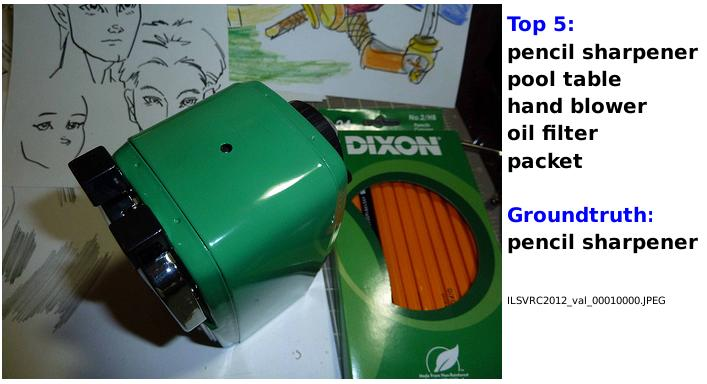
\includegraphics[width=8cm]{figures/classification-problem.jpg}}
    {\centering Image from Pierre Sermanet's slides}
\end{center}

\end{frame}

% -----------------------------------------------------------------------------

\begin{frame}
\frametitle{Taxonomy of Object Recognition}
\framesubtitle{Levels of Recognition -- Localization}

Predict class and location(s) of main object in image

\bigskip
\begin{center}
    \copyrightbox[b]
    {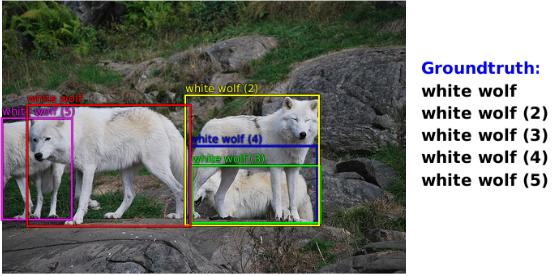
\includegraphics[width=8cm]{figures/localization-problem.jpg}}
    {\centering Image from Pierre Sermanet's slides}
\end{center}

\end{frame}

% -----------------------------------------------------------------------------

\begin{frame}
\frametitle{Taxonomy of Object Recognition}
\framesubtitle{Levels of Recognition -- Detection}

% note that often localization and detection are not separated. for example, face detection is a common term, but in this context it would be localization because there is only one relevant class

Any number of different objects

\bigskip
\begin{center}
    \copyrightbox[b]
    {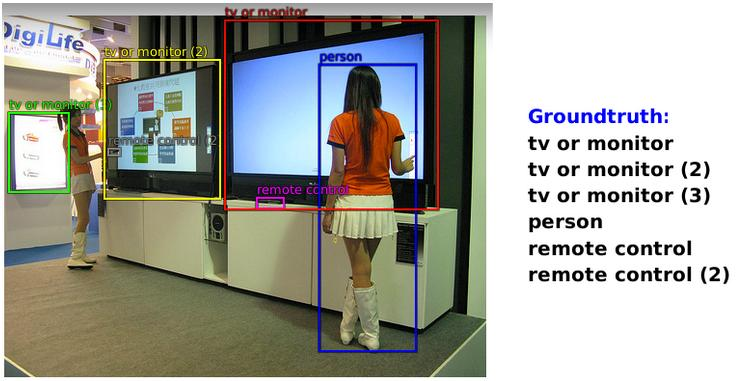
\includegraphics[width=8cm]{figures/detection-problem.jpg}}
    {\centering Image from Pierre Sermanet's slides}
\end{center}

\end{frame}

% -----------------------------------------------------------------------------

\begin{frame}
\frametitle{Challenges}

Instances of same category can look very differently
\begin{itemize}
    \item Illumination, pose, viewpoint, occlusions, background
\end{itemize}

\begin{center}
    \copyrightbox[b]
    {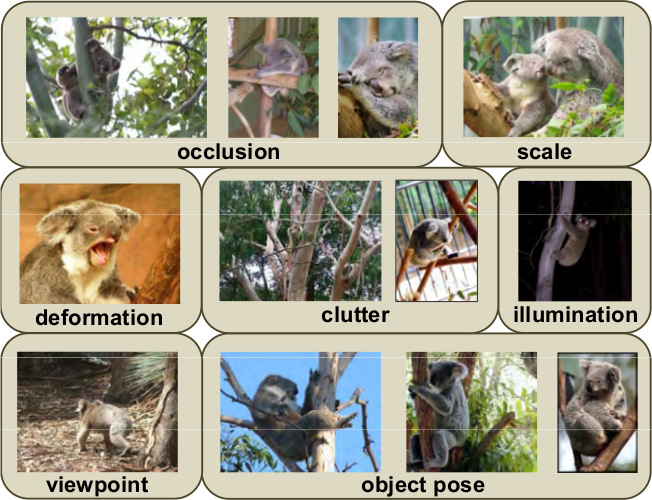
\includegraphics[width=5.5cm]{figures/challenges.jpg}}
    {\centering Image from \cite{grauman2011}}
\end{center}

\end{frame}

% -----------------------------------------------------------------------------

\begin{frame}
\frametitle{Instance Recognition}

\begin{center}
    \copyrightbox[b]
    {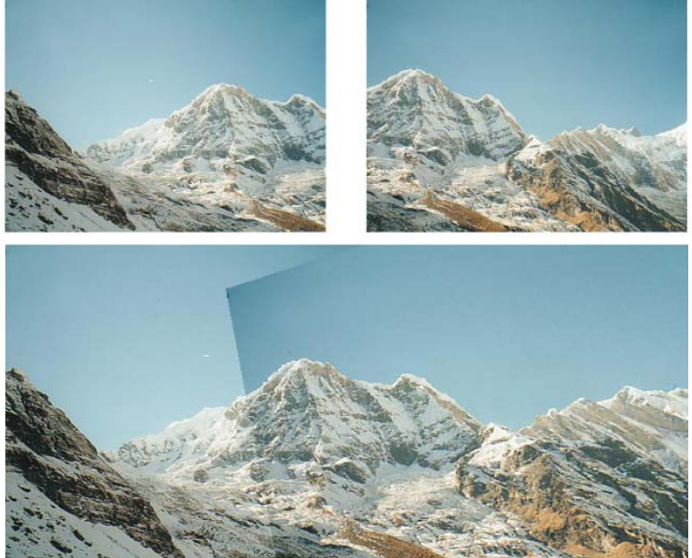
\includegraphics[width=7cm]{figures/panorama-stitching.jpg}}
    {\centering Image adapted from \cite{brown2007}}
\end{center}

\end{frame}

% -----------------------------------------------------------------------------

\begin{frame}
\frametitle{Instance Recognition}

Assume that objects are rigid (nonrigid later) % this is important, because it allows us to perform geometric verification

\bigskip
Often accomplished via \emph{local feature matching}

\bigskip
Given an image of the instance and a search image
\begin{itemize}
    \item Compute local features in both images
    \item Match features between images to find correspondences
    \item Perform geometric verification
\end{itemize}

\end{frame}

% -----------------------------------------------------------------------------

\begin{frame}
\frametitle{Instance Recognition}
\framesubtitle{Local Feature Representations}

Local features form a sparse object representation
\begin{itemize}
    \item Features capture characteristic structure
    \item Allow for efficient matching between images
    \item Representation robust to occlusion and clutter % due to the local features
\end{itemize}

\begin{center}
    \copyrightbox[b]
    {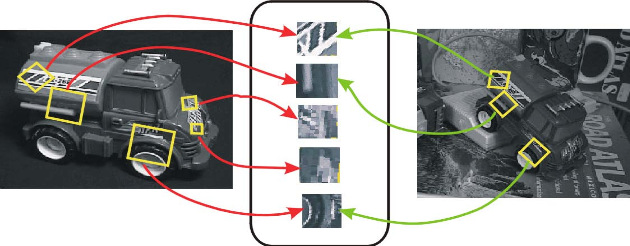
\includegraphics[width=8cm]{figures/local-feature-matching.jpg}}
    {\centering Image from \cite{grauman2011}}
\end{center}

\end{frame}

% -----------------------------------------------------------------------------

\begin{frame}
\frametitle{Instance Recognition}
\framesubtitle{Local Feature Representations}

Many different feature extractors available
\begin{itemize}
    \item SIFT, SURF, BRISK, FREAK, ... % we have covered SIFT shortly in a previous lecture. no more coverage here on the other ones, but they are all quite similar
\end{itemize}

\bigskip
Notes on feature extractor selection
\begin{itemize}
    \item Features should be invariant to expected transformations % like rotation, scale, affine transforms
    \item But not to other transformations % this ensures that the features are as repeatable as possible
    \item Extraction and matching speeds differ % not a problem if object should be searched for in 5 images, but what if in 100.000 images?
\end{itemize}

\end{frame}

% -----------------------------------------------------------------------------

\begin{frame}
\frametitle{Instance Recognition}
\framesubtitle{Feature Matching}

Features are $n$-dimensional vectors
\begin{itemize}
    \item Perform nearest neighbor matching in this feature space
\end{itemize}

\bigskip
Popular matching strategy
\begin{itemize}
    \item Given feature $\vx$ in first image
    \item Find two nearest neighbors $\vy_1,\vy_2$ from second image
    \item $\{\vx,\vy_1\}$ correspond if $\lVert\vx-\vy_1\rVert/\lVert\vx-\vy_2\rVert<0.8$ % y2 is further away from x as y1, hence this fraction is always below 1. the smaller the fraction the smaller the match ambiguity, hence this matching strategy eliminates most false matches / note that this is the Euclidean distance if features in R^n. newer features often use binary descriptors, in which case the Hamming distance is often used for comparison. but this matching strategy still applies
\end{itemize}

\end{frame}

% -----------------------------------------------------------------------------

\begin{frame}
\frametitle{Instance Recognition}
\framesubtitle{Geometric Verification}

Assume that the object in question is planar
\begin{itemize}
    \item Images of planar objects are related by a homography % for nonplanar scenes this is only the case if the camera only zooms or rotates around the center of projection
    \item Also applies to local feature locations
\end{itemize}

\smallskip
\begin{center}
    \copyrightbox[b]
    {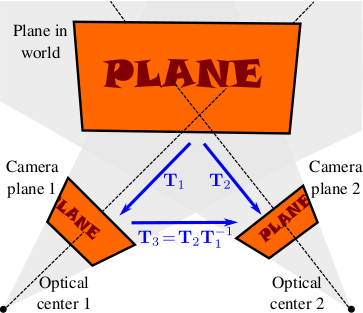
\includegraphics[width=4.5cm]{figures/planar-homography}}
    {\centering Image from \cite{prince12}}
\end{center}

\end{frame}

% -----------------------------------------------------------------------------

\begin{frame}
\frametitle{Instance Recognition}
\framesubtitle{Geometric Verification}

Relation allows for detecting erroneous correspondences
\begin{itemize}
    \item Estimate homography $T$ from correspondences % using some robust method, like RANSAC
    \item Discard correspondences for which $\lVert\vx-T(\vy_1)\rVert>t$ % t is some small threshold that depends on the data, usually a few pixels
\end{itemize}

\bigskip
Verification also possible for nonplanar scenes
\begin{itemize}
    \item Epipolar geometry constraints (previous lecture) % basically, if we know the intrinsics we can estimate the relative camera positions/orientations, which is all we need as discussed in the previous lecture. if we dont know the intrinsics, this is still possible by computing the fundamental matrix. this is out of scope here, but see any of the CV books referenced below if interested
\end{itemize}

\end{frame}

% -----------------------------------------------------------------------------

\begin{frame}
\frametitle{Instance Recognition}
\framesubtitle{Applications -- Object Detection}

Detection and pose estimation of rigid objects

\bigskip
\begin{center}
    \copyrightbox[b]
    {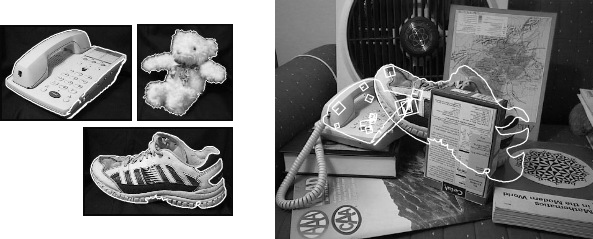
\includegraphics[width=8cm]{figures/rigid-object-detection.jpg}} % note the occlusions and transformations
    {\centering Image adapted from \cite{lowe2004}}
\end{center}

\end{frame}

% -----------------------------------------------------------------------------

\begin{frame}
\frametitle{Instance Recognition}
\framesubtitle{Applications -- Object Detection}

Industrial applications like PCB recycling

\bigskip
\begin{center}
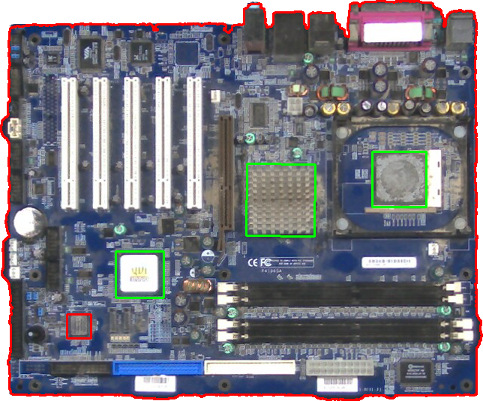
\includegraphics[width=5.5cm]{figures/reclaim-pcb.jpg}
\end{center}

\end{frame}

% -----------------------------------------------------------------------------

\begin{frame}
\frametitle{Instance Recognition}
\framesubtitle{Applications -- Panorama Stitching}

\begin{center}
    \copyrightbox[b]
    {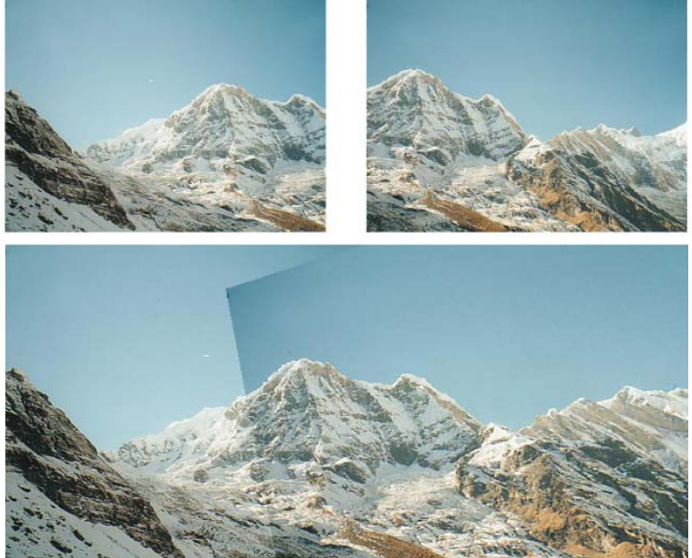
\includegraphics[width=7cm]{figures/panorama-stitching.jpg}}
    {\centering Image adapted from \cite{brown2007}}
\end{center}

\end{frame}

% -----------------------------------------------------------------------------

\begin{frame}
\frametitle{Face Localization}

\begin{center}
    \copyrightbox[b]
    {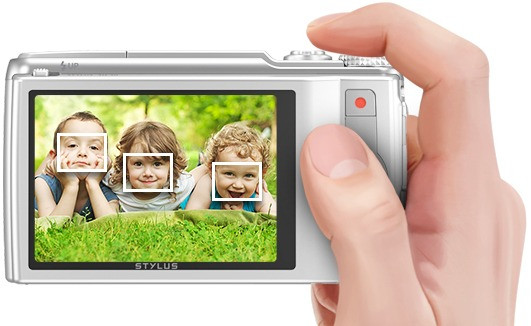
\includegraphics[width=7cm]{figures/camera-faces.jpg}}
    {\centering Image from \url{olympus-europa.com}}
\end{center}

\end{frame}

% -----------------------------------------------------------------------------

\begin{frame}
\frametitle{Face Localization}

Many applications, such as
\begin{itemize}
    \item Smart cameras (autofocus on faces)
    \item Security (preprocessing step to face recognition)
    \item Augmented reality \& gaming
\end{itemize}

\bigskip
We focus on the popular method from [\cite{viola2001}]
\begin{itemize}
    \item Fast enough to run on e.g.\ cameras
\end{itemize}

\end{frame}

% -----------------------------------------------------------------------------

\begin{frame}
\frametitle{Face Localization}
\framesubtitle{\cite{viola2001} -- Approach}

Sliding window approach % we don't know where the faces might be, so we just scan over the whole image. note that the window size depends on the expected size of the faces, and as such is not scale invariant (but we could repeat the test with different scales)
\begin{itemize}
    \item Slide window over image % note that this results one classification per pixel (unless we chose some offset), and the classification is binary ... w denotes whether a face is present
    \item Infer label $w\in\{0,1\}$ based on measurements $\vx$ % of the current window
    \item Perform non-maximum suppression of confidence scores % we also get some form of confidence along with the label (similar to the probabilistic models we discussed, but they are not probabilities), which is mandatory for this method to work
\end{itemize}

\medskip
\begin{center}
\begin{tikzpicture}
\node [inner sep=0pt,above right]{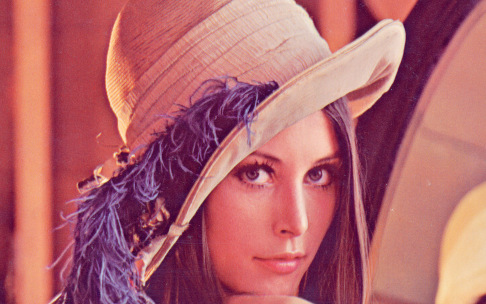
\includegraphics[width=5cm]{figures/lena.jpg}};;
\draw[thick,green,opacity=0.2] (1.6,0.25) rectangle (3.6,2.25);
\draw[thick,green,opacity=0.4] (1.7,0.25) rectangle (3.7,2.25);
\draw[thick,green,opacity=0.6] (1.8,0.25) rectangle (3.8,2.25);
\draw[thick,green,opacity=0.8] (1.9,0.25) rectangle (3.9,2.25);
\draw[thick,green] (2,0.25) rectangle (4,2.25);
\end{tikzpicture}
\end{center}

\end{frame}

% -----------------------------------------------------------------------------

\begin{frame}
\frametitle{Face Localization}
\framesubtitle{\cite{viola2001} -- Features}

Simple features -- difference $d$ in rectangular subwindow of $\vx$
\begin{itemize}
    \item Can be computed in constant time using integral images
    \item Limited number of such features $\{f_t\}_{t=1}^T$
\end{itemize}

\bigskip
\begin{center}
    \copyrightbox[b]
    {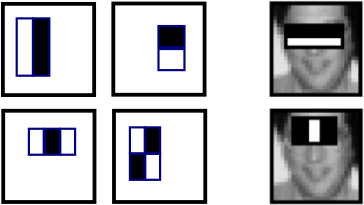
\includegraphics[width=5cm]{figures/vj-features.png}}
    {\centering Image adapted from \cite{prince12}}
\end{center}

\end{frame}

% -----------------------------------------------------------------------------

\begin{frame}
\frametitle{Face Localization}
\framesubtitle{\cite{viola2001} -- Classifier}

Classification using a cascading classifier
\begin{itemize}
    \item Cascade of $K\leq T$ weak but fast classifiers $c_k=f_k>t_k$
    \item Early rejection of non-face windows for speed % we just abort as soon as the patch is not classified as a face
    \item Final classifier is $C(\vx)=\text{sign}(w_0+\sum_k w_kc_k)$ % w are some learned weights
\end{itemize}

\medskip
\begin{center}
    \copyrightbox[b]
    {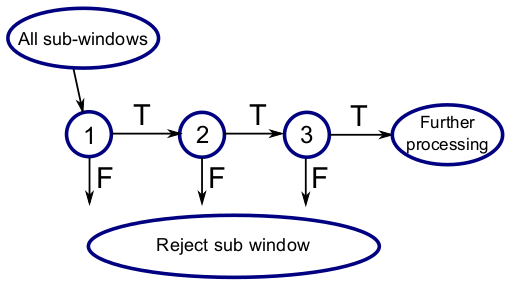
\includegraphics[width=5cm]{figures/boosting-cascade}}
    {\centering Image from \cite{prince12}}
\end{center}

\end{frame}

% -----------------------------------------------------------------------------

\begin{frame}
\frametitle{Face Localization}
\framesubtitle{\cite{viola2001} -- Classifier}

Subset of $K$ classifiers, order, and weights $w$ are learned

\bigskip
Accomplished via \emph{boosting} -- for each $k=1\cdots K$
\begin{itemize}
    \item Find best classifier according to training set, set as $c_k$ % this is the classifier that, if added to the current C(x), leads to the biggest reduction in error
    \item Raise weights of samples misclassified by current $C$
\end{itemize}

\bigskip
\begin{center}
    \copyrightbox[b]
    {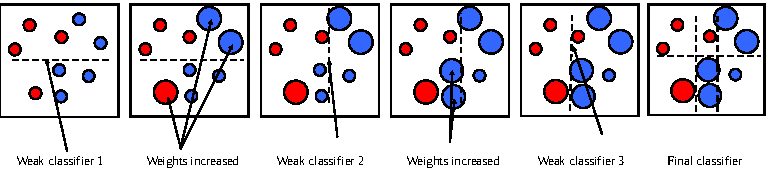
\includegraphics[width=10cm]{figures/boosting.pdf}} % see Szeliski's book for a good explanation
    {\centering Image from \cite{szeliski2010}}
\end{center}

\end{frame}

% -----------------------------------------------------------------------------

\begin{frame}[allowframebreaks=0.8]
\frametitle{Bibliography}

\printbibliography

\end{frame}

\end{document}
